\documentclass[11pt,a4paper]{article}
\usepackage[T1]{fontenc}
\usepackage[utf8]{inputenc}
\usepackage{lmodern,amsmath,amssymb,amsthm,mathtools,booktabs,longtable,array,geometry,tikz,hyperref}
\usetikzlibrary{arrows.meta,positioning,calc,fit}
\geometry{margin=28mm}
\hypersetup{colorlinks=true,linkcolor=blue!55!black,citecolor=blue!55!black,urlcolor=blue!55!black}
\newtheorem{theorem}{Theorem}[section]
\newtheorem{proposition}[theorem]{Proposition}
\newtheorem{lemma}[theorem]{Lemma}
\newtheorem{corollary}[theorem]{Corollary}
\theoremstyle{definition}\newtheorem{definition}[theorem]{Definition}\newtheorem{example}[theorem]{Example}
\theoremstyle{remark}\newtheorem{remark}[theorem]{Remark}
\newcommand{\cl}{\mathcal K}
\newcommand{\pare}{\operatorname{pare}}
\newcommand{\Ind}{\operatorname{Ind}}
\newcommand{\im}{\operatorname{im}}
\newcommand{\NN}{\mathbb N}
\newcommand{\Z}{\mathbb Z}
\newcommand{\cprod}{\mathbin{\lor}}
\newcommand{\D}{\mathcal D}
\newcommand{\F}{\mathcal F}
\newcommand{\code}[1]{\texttt{#1}}
\title{Clique dynamics and topology of complements of cubic graphs\\\large A census and methods for implicit iterates}
\author{Research survey and computational record}
\date{26 November 2026}
\begin{document}
\maketitle
\begin{abstract}
We survey the investigation of clique behavior and clique-complex homotopy types of complements of cubic graphs, concentrating on order fourteen. The recovered ledger of all 540 inputs (509 connected cubic graphs and 31 disconnected ones) records 502 divergent, 18 clique-null and 20 undetermined complements. Four of the positive records have not been independently replayed in the recovered ledger. The homotopy ledger records exact wedge types for the original and first clique graphs on all 540 inputs. We develop coaffine stable-image criteria, a necessary-and-sufficient incidence-cut characterization of octahedral retractions (including special octahedra), symbolic lifting and obstructions, Helly-defect bounds, and ranked replacement templates for implicit paring. These tools yield large but finite growth bounds, exact negative results for specified certificate classes and a certified lower bound of 102,516,282 simultaneous dominated deletions in the third-level precursor of graph 182. None of those latter results decides the behavior of the remaining twenty graphs. The accompanying Org workbook distinguishes blind package searches from historical certificate replay.
\end{abstract}
\tableofcontents
\section{Background and notation}
All graphs are finite, simple and nonempty. A \emph{complete} is a nonempty pairwise adjacent set; a \emph{clique} is an inclusion-maximal complete. Write \(\cl(X)\) for the clique family, and identify each vertex \(q\in V(K(X))\) with its support \(T_q\in\cl(X)\). The clique graph \(K(X)\) is the intersection graph of this family. Write \(K^0(X)=X\), \(K^{j+1}(X)=K(K^j(X))\). Convergence means that the iterates have bounded order (equivalently, the sequence is eventually periodic up to isomorphism); divergence means that the orders tend to infinity. A graph is clique-null if some actual iterate is a point. A graph is clique-Helly when every pairwise intersecting subfamily of its cliques has nonempty intersection. The Helly condition implies clique-convergence \cite{escalante}; it is not necessary.

Let \(C\) be a cubic graph, i.e., all degrees equal three, and \(G=\overline C\). The clique complex \(\Delta(G)\) has as faces all completes and the empty face. In this case \(\Delta(G)=\Ind(C)\), the independence complex. The complement of a cubic graph on at least 14 vertices is not clique-Helly by \cite[Theorem 5.1]{regular}; the bound is sharp at order twelve. The earlier LAGOS draft \cite{lagos} studies the small cubic census and the topological questions that motivate this work. The 2023 paper also conjectures the existence of clique-convergent cubic complements of unbounded order. The census here is finite evidence, not a proof of that conjecture.

We use weak graph morphisms: if \(uv\in E(X)\), then \(f(u)=f(v)\) or \(f(u)f(v)\in E(Y)\). A retraction onto an induced subgraph \(Y\subseteq X\) is a morphism \(r:X\to Y\) fixing every vertex of \(Y\). A vertex \(v\) is dominated by a distinct vertex \(w\) if \(N_X[v]\subseteq N_X[w]\); deleting \(v\) is an ordinary fold. A graph with no such pair is stiff. Set
\[
 P_0(G)=\pare(G),\qquad P_{j+1}(G)=\pare(K(P_j(G))),
\]
where paring means repeated ordinary folds to a stiff graph. A choice of labels and fold order is part of a computational certificate; the results on behavior and homotopy are label independent.

\begin{lemma}[Retraction and paring]\label{lem:pare}
A retraction \(X\to Y\) induces a retraction \(K(X)\to K(Y)\), and hence divergence of \(Y\) implies divergence of \(X\). Ordinary folds preserve clique behavior and the homotopy type of the clique complex. In particular, \(P_j(G)\) is (up to labeling) a retract of \(K^j(G)\); if \(P_j(G)\) is a point, then \(G\) is clique-null.
\end{lemma}
\begin{proof}
For a clique of \(X\), extend its image under the retraction to a clique of \(Y\); intersections are preserved. For each clique of \(Y\) choose an extension to a clique of \(X\). On these choices the composite is the identity by maximality, proving the first assertion. For a fold, every clique containing the deleted vertex contains its dominator. Extend the cliques of the reduced graph back to the original graph; the clique-graph vertices not chosen for the extensions are dominated by extensions of their restricted supports (intersection at the removed vertex also implies intersection at its dominator). Thus a fold induces a sequence of folds on the clique graph. The topology assertion follows by the elementary strong collapse: the link of the removed vertex is a cone with apex its dominator. Preservation of clique-convergence and clique-nullity under paring is the dismantling theorem of \cite{dismantling}; see also \cite{contraction,collapses}. The iterative retraction claim follows by induction. We use the cited dismantling theorem for the final clique-null assertion, not merely the existence of a retraction onto a point (which alone would be vacuous).
\end{proof}

\section{Census, topology and status of the computations}\label{sec:census}
The connected cubic graph lists at orders 8, 10, 12 and 14 have 5, 19, 85 and 509 entries \cite{hog}. The disconnected cases are constructed by disjoint unions of connected cubic graphs of order at least four. At order fourteen the partitions are \(4+10\), \(6+8\), \(4+4+6\), giving \(19+2\cdot5+2=31\). Throughout, a bare integer denotes the one-based position in the original connected cubic graph6 file \code{cub14.g6}; \(G_i\) denotes its complement, not the cubic graph itself. The frozen Git blob is \code{0a2e0fb60b4fc9414b7b195fc53b771ebbc031f1}. Disconnected identifiers record the component orders and indices, for example \code{6+8:2:3}. The Org companion gives the full behavior grouping.

\begin{table}[ht]
\centering
\begin{tabular}{rrrrrl}\toprule
Order & All & Connected & Convergent & Divergent & Unresolved\\\midrule
4 &1&1&1&0&0\\
6 &2&2&2&0&0\\
8 &6&5&6&0&0\\
10 &21&19&4&17&0\\
12 &94&85&1&80&13\\
14 &540&509&18&502&20\\\bottomrule
\end{tabular}
\caption{Small-order historical results from \cite{lagos}, and the recovered order-14 ledger. The order-12 line is the draft baseline, not a claim that all later work has been replayed. The later predecessor record narrowed its unresolved set to two, but a complete updated per-graph ledger for order 12 was not recovered here.}
\end{table}
The order-14 ledger records 396 expansive witnesses at depth zero, 72 additional ones at depth one, and 34 at depth two (including four carried-forward records). The 18 convergences are all clique-null: five point reductions at depth one and thirteen at depth two. There are 471 divergent connected-cubic complements recorded, 18 null and 20 unresolved; all 31 disconnected-cubic complements are recorded divergent. In the strict recovered-certificate accounting, 498 divergent records have a reported replay, four further positive records (150,252,270,472) are historical only, and 20 remain undetermined. This survey has not independently replayed every archived computation.

\begin{center}
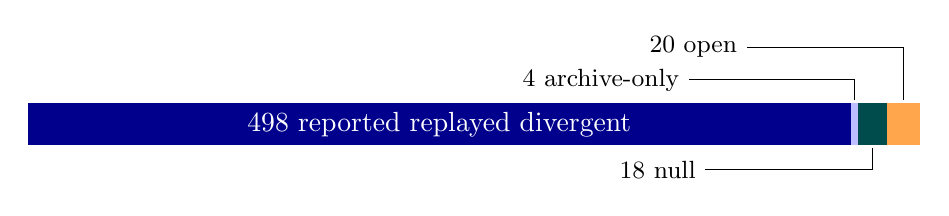
\begin{tikzpicture}[x=0.021cm,y=0.75cm]
\fill[blue!55!black] (0,0) rectangle (498,0.7);
\fill[blue!25] (498,0) rectangle (502,0.7);
\fill[teal!60!black] (502,0) rectangle (520,0.7);
\fill[orange!70] (520,0) rectangle (540,0.7);
\node[white] at (249,.35) {498 reported replayed divergent};
\draw (500,.75)--(500,1.1)--(400,1.1) node[left,font=\small]{4 archive-only};
\draw (511,-.05)--(511,-.42)--(410,-.42) node[left,font=\small]{18 null};
\draw (530,.75)--(530,1.65)--(435,1.65) node[left,font=\small]{20 open};
\end{tikzpicture}
\end{center}
The exact unresolved list is
\[
\begin{gathered}
94,127,182,185,206,283,287,320,344,363,368,\\
441,442,451,462,473,497,506,508,509.
\end{gathered}
\]
The null cases at depth one are 27, 400, 405, 406, 416; at depth two they are 57, 85, 129, 144, 156, 158, 169, 408, 415, 417, 421, 448, 482. These lists and the data provenance are included in the companion workbook.

\subsection{Homotopy classification}
For a finite family of cliques, \(\Delta(G)\) is covered by its facet simplices. Their nonempty intersections are contractible, so the nerve theorem identifies \(\Delta(G)\) up to homotopy with the nerve of this cover. This nerve has one vertex per clique but is not in general \(\Delta(K(G))\): the latter fills all pairwise intersecting families, whereas the nerve requires total intersection. They coincide when \(G\) is clique-Helly. This explains why the topology can change under \(K\).

For homotopy computations we use ordinary folds, vertex and edge simplicial collapses, the join decomposition \(\Ind(C\sqcup D)=\Ind(C)*\Ind(D)\), acyclic matching on the face poset (Forman \cite{forman}, Dong \cite{dong}), symbolic integral Morse computations and spherical generation. A matching is acyclic if reversing its matched Hasse arrows creates no directed cycle; it gives a CW model with cells indexed by unmatched faces. If one critical vertex remains and all other critical cells have the same positive dimension, the model is a wedge of spheres. For consecutive critical dimensions \(d,d+1\), \(d\ge2\), the lower skeleton is a wedge of \(d\)-spheres. By Hurewicz, an attaching map of a \((d+1)\)-cell is null if its integral cellular boundary is zero. For \(d=1\) with one circle the same statement holds by degree; with several circles the commutator illustrates why vanishing homology boundary alone does not suffice. More generally a certificate of simple connectivity and integral spherical generators for all positive homology groups, with no torsion and the right ranks, gives a homology equivalence from the corresponding wedge, and Whitehead's theorem gives a homotopy equivalence \cite{hatcher}. These tests require actual attaching-map or spherical-generation justification, not only Betti numbers. Steenrod-square calculations may obstruct a proposed wedge, but the vanishing of a particular square alone is not a wedge proof.

The archived homotopy-transition table reports exact wedges for both \(\Delta(G_i)\) and \(\Delta(K(G_i))\) for all 540 inputs, with 19 unchanged types, 28 contractible original complexes and 22 contractible first-iterate complexes. There are 521 changed types. The 19 equal types are all contractible, including the exceptional unresolved graph 182. These numbers are aggregated from \nolinkurl{cubic14_complete_homotopy_transitions.csv}; the original CSV and the twelve final certificates are project archives, not all accessible for byte-level replay here. A wedge of zero spheres in the sense of zero \emph{summands} denotes a point. Examples:
\begin{center}\begin{tabular}{rlll}\toprule
ID & \(\Delta(G_i)\) & \(\Delta(K(G_i))\) & Behavior\\\midrule
1 & \(2S^2\vee S^3\)&\(4S^3\vee4S^4\vee S^7\)& divergent\\
27&point&point&null\\
94&\(S^2\)&\(\bigvee_3 S^4\)&open\\
182&point&point&open\\
308&\(S^3\)&\(S^4\)&divergent\\
379&point&\(S^5\)&divergent\\
441,442,451&\(S^3\)&\(S^5\)&open\\
509&\(\bigvee_6 S^3\)&\(\bigvee_{36}S^5\)&open\\\bottomrule\end{tabular}\end{center}
Here \(mS^j\) is shorthand for a wedge of \(m\) copies of \(S^j\). Thus contractibility of \(G\) alone does not imply convergence (e.g. 379); neither contractibility of \(K(G)\) nor an induced octahedron decides the eventual behavior. The order-twelve examples 48 and 81, with cubic codes \verb|K{O_ogG@GC_L| and \verb|KsX@?gQA?H_Y|, have contractible original clique complexes and first clique complexes homotopic to \(S^3\) in the recovered study. They should not be conflated with the two residual cases of a different behavior census without an explicit ID match.

\section{Coaffine maps and expansive stable images}\label{sec:coaffine}
A coaffine endomorphism is a weak morphism \(f:X\to X\) such that \(f(v)\notin N_X[v]\) for all vertices. A bijective such map is a coaffination (an automorphism); the expansive-graph literature uses coaffine pairs with a specified coaffination and admissible, i.e. equivariant, morphisms \cite{expansive,relations}. We use the following results of \cite[Theorems 2.4, 3.6, 4.6]{expansive}: expansivity transfers along an admissible morphism from an expansive pair, the join of three nonempty coaffine pairs is expansive, and the join of two is expansive if one factor is connected. Expansivity implies divergence. These are stronger than ordinary non-equivariant induced-subgraph containment.
\begin{proposition}[Stable image]\label{prop:stable}
Let \(f\) be coaffine on \(X\). For sufficiently large \(m\), \(R=f^m(X)\) is stable and \(f|_R\) is a coaffination. Some power of \(f\) is a retraction onto \(X[R]\). If \(R\) contains two nonempty disjoint invariant completely joined sets, one inducing a connected graph, or three pairwise completely joined nonempty invariant sets, then \(X\) is divergent.
\end{proposition}
\begin{proof}
The descending images stabilize since the graph is finite. On the stable set \(f\) is a permutation preserving edges, hence an automorphism. Choose an exponent at least the stabilization time and divisible by its permutation order. The power fixes the stable set and maps everything into it. Each invariant subset carries a coaffination; its union with the other factors is an expansive coaffine subgraph by the cited join theorems. Its inclusion in the stable image is admissible. Apply expansivity transfer, then the retraction theorem.
\end{proof}
\begin{corollary}[Connected invariant summand test]
If \(A,B\subseteq V(X)\) are disjoint nonempty forward-invariant completely joined sets and there is a path in \(X[B]\) from some \(u\) to \(f(u)\), then \(X\) diverges.
\end{corollary}
\begin{proof}
In the stable image the mapped path is a weak walk connecting \(f^m(u)\) and \(f^{m+1}(u)\). Its component in \(f^m(B)\) is invariant under the automorphism. Apply Proposition~\ref{prop:stable} to that component and \(f^m(A)\).
\end{proof}
A coaffine CSP has domains \(D(v)=V(X)\setminus N_X[v]\) and for each edge \(uv\) forbids nonadjacent distinct images. Arc consistency deletes a value when no compatible value remains in a neighbor's domain; singleton tests temporarily fix a value and apply the same exact propagation. Both are safe, but not complete without branching. In SAT, variables \(x_{uv}\) encode assignments, exactly one per source. Invariant sets can be selected by color variables and implications \(c_{u,i}\land x_{uv}\Rightarrow c_{v,i}\). Pairwise complete joins are encoded by prohibiting differently colored nonedges. Sharing disjunctions and incidence factors reduces clause counts without changing the feasible maps. An exhaustive negative result excludes only the specified predicate.
\begin{lemma}[Obstruction by non-coaffinity]
If \(X\) admits no coaffine endomorphism, it has no retract admitting one.
\end{lemma}
\begin{proof}
For a retraction \(r:X\to Y\) and coaffine \(g:Y\to Y\), the composite \(igr\) (where \(i\) includes \(Y\)) is a morphism. If \(igr(v)\in N_X[v]\), applying \(r\) contradicts coaffinity of \(g\) at \(r(v)\).
\end{proof}
For example \(O_1*C_5\) is expansive by the connected summand theorem even though a three-summand decomposition need not be available. The two factors have the antipodal swap and the rotation by two, respectively. The general method accepts stable images with complement components other than edges, including cycle complements. In the historical stage-zero and stage-one searches the acceptance predicate was an expansive invariant subjoin, not merely existence of a coaffine map. The production solver for arbitrary coaffine maps may stop at a nonexpansive map; this is an important reproducibility gap addressed in the workbook.

\section{Octahedra and the incidence-cut theorem}\label{sec:cuts}
Put \(O_d=\overline{dK_2}\), with opposite pairs \((a_i,b_i)\). Its cliques choose one endpoint from each pair, and the only disjoint clique is the complementary transversal. Hence \(K(O_d)\cong O_{2^{d-1}}\), so \(O_d\) is divergent for \(d\ge3\). Its clique complex is a join of \(d\) copies of \(S^0\), namely \(S^{d-1}\). Retraction onto it also gives a split integral homology summand in degree \(d-1\), a useful necessary condition for prescribed targets.
\begin{proposition}[Special octahedra are retracts]\label{prop:special}
If an induced \(O_d\subset X\) has a transversal \(\{a_1,\ldots,a_d\}\) which is a clique of \(X\), then \(O_d\) is an ordinary retract of \(X\).
\end{proposition}
\begin{proof}
Fix all target vertices. For every other vertex \(v\), maximality of the transversal gives an \(a_i\) nonadjacent to \(v\); send \(v\) to \(b_i\). The only forbidden image pairs are \(a_i,b_i\). Since only \(a_i\) itself maps to \(a_i\), the choice ensures no edge maps to such a pair. This proves the retraction. In particular the special criterion is not an independent divergence mechanism.
\end{proof}
\begin{theorem}[Incidence-cut characterization]\label{thm:cut}
Let \(X\) be the intersection graph of nonempty supports \(F_v\subseteq U\). Let \((a_i,b_i)\), \(1\le i\le d\), induce \(O_d\). There is a retraction onto this target if and only if there are subsets \(C_i\subseteq U\) with
\[
 F_{a_i}\subseteq C_i,\quad F_{b_i}\cap C_i=\varnothing,\quad
 \forall v\ \exists i\ (F_v\subseteq C_i\ \text{or}\ F_v\cap C_i=\varnothing).
\]
\end{theorem}
\begin{proof}
From a retraction take \(C_i=\bigcup_{r(v)=a_i}F_v\). Opposite fibers are disjoint in incidence because an edge cannot map to opposite endpoints. Conversely, fix all endpoints and assign each other support to an anchor on a shore containing its entire support. Two intersecting supports cannot map to opposite shores of one cut, which proves the morphism property.
\end{proof}
In particular \(C_i=F_{a_i}\) realizes the special-octahedron case. A set of pairs is an induced matching in \(H=\overline X\). For any retract its endpoints must meet every open neighborhood of \(H\): compose with the target antipodal involution to obtain a coaffine map \(f\) with \(f^3=f\), \(f^2=r\). Conversely such a map with octahedral image gives a retraction by squaring. This observation supports both direct coaffine search and the incidence SAT encoding. A support with no disjoint target endpoint obstructs every cut system for that matching.

\begin{figure}[ht]\centering
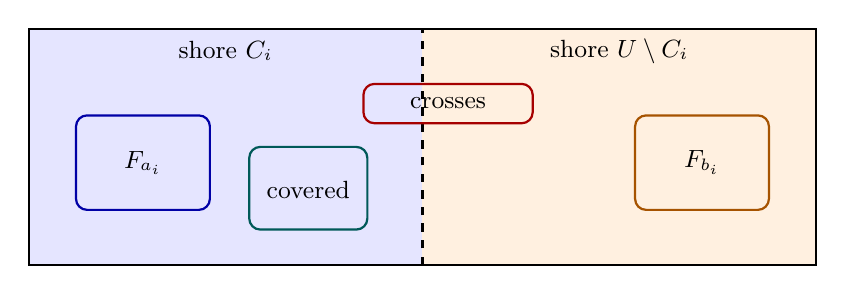
\begin{tikzpicture}[every node/.style={font=\small}]
\fill[blue!10] (0,0) rectangle (5,3);\fill[orange!12] (5,0) rectangle (10,3);
\draw[thick] (0,0) rectangle (10,3);\draw[dashed,thick] (5,0)--(5,3);
\node at (2.5,2.72) {shore \(C_i\)};\node at (7.5,2.72) {shore \(U\setminus C_i\)};
\draw[blue!65!black,thick,rounded corners] (.6,.7) rectangle (2.3,1.9);
\draw[orange!65!black,thick,rounded corners] (7.7,.7) rectangle (9.4,1.9);
\node at (1.45,1.3) {\(F_{a_i}\)};\node at (8.55,1.3) {\(F_{b_i}\)};
\draw[teal!70!black,thick,rounded corners] (2.8,.45) rectangle (4.3,1.5);
\node at (3.55,.95) {covered};
\draw[red!65!black,thick,rounded corners] (4.25,1.8) rectangle (6.4,2.3);
\node at (5.325,2.05) {crosses};
\end{tikzpicture}
\caption{One incidence cut. A crossing support must be covered by a different cut.}\end{figure}

A weighted improvement of a single cut is a min-cut problem. Pin the first anchor to the source and its mate to the sink. For each support that can fit on the left create a reward node joined from the source by its weight and to each of its atoms by an effectively infinite capacity; use the reverse construction for the right. A reward is earned exactly when the entire support lies on that shore. Choosing capacity above the sum of all finite weights gives the maximum total covered weight. Iterating weighted updates, replacing incompatible pairs and emphasizing uncovered supports yields a useful heuristic, not an exact existence test.

\subsection{Exact filters and local repairs}
For a proposed pair \(ab\) let \(U_{ab}\) contain its endpoints and the endpoints of every other candidate pair compatible with it. In the coaffine formulation restrict each domain to \(N_H(v)\cap U_{ab}\). An empty domain excludes the pair. If sources forced to map to \(a\) and to \(b\) have intersecting support unions, the pair is impossible. Repeating after pair eliminations remains safe. For a fixed selected endpoint set \(S\), if adjacent sources have singleton domains at opposite endpoints, the matching is invalid. The resulting clause in the selection variables says that at least one of the two anchors must be absent or one source must gain an alternative selected endpoint.

A more general fixed-target obstruction is obtained from a complete \(W\) whose intersection constraints force inconsistent shores. Exact SAT can extract a core of source supports. A master problem selects induced matching pairs and covers a finite sample of supports; a subproblem tests all supports. An UNSAT core contributes at least one previously absent support (otherwise the master assignment would already satisfy that core). With no resource limits this finite refinement terminates. Regional searches retain a subset of pairs and allow all other pairs and cuts to vary. A core of retained pairs must be hit by the set of abandoned pairs, turning repeated failures into a hypergraph transversal bound. For the recovered near-targets below the minimum certified abandonment bounds were 4, 2 and 2 respectively. These are necessary changes, not sufficient repairs.

\subsection{A positive depth-two certificate: graph 308}
The cubic graph6 code is \verb|M{O_o_G@_G_K?W?B_|. Reconstructing its pared iterates gives \(|P_1|=35\), and \(K(P_1)\) has 577 cliques. Paring leaves 571 supports and 146,127 edges. The recovered 22 cuts give zero uncovered supports and compatible anchors, proving \(P_2\to O_{22}\) and therefore divergence. The archived discovery used seed 137, 250,000 steps, reaching the witness at step 118,644. In this survey preparation we independently reconstructed the support labels (lexicographic clique order at level one, numeric mask order at level two), and verified all 22 anchor constraints, induced matching and full coverage from graph6. The companion includes the 22 masks and package-based replay, separate from blind search. It is not necessary to generate \(K(P_2)\).

\section{Implicit third iterates and finite growth}\label{sec:implicit}
The obstacle in the remaining cases is the order of \(K(P_2)\), not simply its edge count. Let \(X=P_2\) and \(H=\overline X\). Boolean variables \(z_v\) encode a clique of \(X\) by clauses
\[
 (\neg z_u\lor\neg z_v)\ (uv\in E(H)),\qquad
 z_v\lor\bigvee_{w\in N_H(v)}z_w\ (v\in V(H)).
\]
The first group asserts independence in \(H\), the second maximality. One can test disjointness, required intersections, or coverage without enumerating the maximal independent sets. For a fixed system of incidence cuts, an uncovered clique exists exactly when there is a complete meeting both shores of every cut: a complete extends to a clique, and crossing persists on extension. Thus maximality clauses may be omitted from this particular UNSAT query. For arbitrary coaffine maps, the region formulation in Section~\ref{sec:defect} is useful.

The archived implicit searches gave induced octahedra at depth three of dimensions 200, 902, 111, 153, 99, 116, 595 and 269 for IDs 94, 182, 185, 206, 283, 320, 441 and 451. For 182, component switches increased the bound to 904. If \(O_d\) is merely induced in a graph, its \(2^d\) transversals extend to distinct maximal completes (two distinct transversals disagree on some opposite pair). This proves a finite lower bound at the next iterate, not eventual divergence. In particular \(|K^4(G_{182})|\ge 2^{904}\). All eight original target families had a clique meeting all endpoints, so none of those particular induced octahedra could be a retract.

\subsection{Switching disjoint cliques}
For disjoint cliques \(A,B\) of \(X\), the complement of \(X[A\cup B]\) is bipartite. Interchanging the two shores independently in its connected components gives new pairs of disjoint completes. If each component has both shores nonempty, fixing one component and switching \(k\) others gives \(2^k\) pairs with cross-pair intersections (two distinct switches agree on the fixed component and disagree on at least one switched component). If the resulting completes are maximal, this is an induced \(O_{2^k}\) in \(K(X)\). Maximality and compatibility with other pairs must be checked, not inferred from switching alone.

\section{Partial retractions, symbolic lifts and their obstructions}\label{sec:lift}
Three particularly good near-solutions were reconstructed and checked in the archived labels:
\begin{center}\begin{tabular}{rrrrr}\toprule
ID & \(|P_1|\)&\(|P_2|\)& target & uncovered supports\\\midrule
441&28&372&\(O_{21}\)&2\\
442&33&518&\(O_{24}\)&2\\
451&32&551&\(O_{27}\)&1\\\bottomrule\end{tabular}\end{center}
These give genuine partial retractions after deleting the uncovered vertices, not global ones. The exact local repairs (561 fixed-anchor and 1,353 fixed-cut regions) were negative. Enlarging the target of 451 by its exceptional vertex yielded \(O_{25}*\overline{P_5}\), but there was an empty domain. Adding the next offending vertex yielded \(O_{25}*\overline{P_6}\); SAT excluded it and all 495 one-vertex extensions failed propagation. For 442, fourteen retractions onto enlarged targets were found, but all targets were clique-null; a retract onto a clique-null graph does not show clique-nullity of the host. If \(Q\) is coaffine and \(k\ge2\), \(O_k*Q\) is expansive by the three-summand theorem. If \(K(Q)\) is coaffine and \(k\ge3\), then \(K(O_k*Q)\cong O_{2^{k-1}}\cprod K(Q)\) (disjunctive product); combining antipodal and coaffine maps yields two completely joined invariant groups of first-factor antipodal pairs, one connected. The case \(k=2\) requires a separate connectedness condition for this second argument.

\begin{theorem}[Partial-retraction lift]\label{thm:partial}
Suppose \(r:X-D\to O_d\) is a retraction onto a target disjoint from \(D\). If no vertex of \(D\) is adjacent to every target vertex, then \(K(X)\) contains an induced \(O_{2^{d-1}}\).
\end{theorem}
\begin{proof}
For each binary orientation \(\varepsilon\in\{0,1\}^d\), let \(T_\varepsilon\) be its target transversal and choose any maximal extension \(Q_\varepsilon\) in \(X\). Noncomplementary distinct orientations share an anchor. Complementary extensions cannot intersect outside \(D\), since such an intersection would map under \(r\) to both complementary target transversals. They cannot intersect in \(D\) by the hypothesis. Distinct orientations give distinct extensions since their union contains an opposite pair. Therefore the indicated induced octahedron exists.
\end{proof}
Even when the hypothesis on \(D\) fails, define \(\mathcal B_F\) to be the orientations with a maximal extension avoiding \(F\subseteq D\). A complementary pair has disjoint maximal extensions exactly when some \(F\subseteq D\) satisfies \(\varepsilon\in\mathcal B_F\), \(\bar\varepsilon\in\mathcal B_{D\setminus F}\). Indeed intersections outside \(D\) remain impossible. For each excluded vertex choose a nonneighbor to block it; the blockers must be pairwise compatible and compatible with the transversal. This describes \(\mathcal B_F\) by a union of Boolean subcubes. Counting the union by recursive conditioning gives the following certified induced dimensions:
\begin{center}\begin{tabular}{rrrr}\toprule
ID& maximum candidate pairs&liftable pairs& subcubes\\\midrule
441&1,048,576&425,984&64\\
442&8,388,608&7,953,920&20\\
451&67,108,864&67,108,864&16\\\bottomrule\end{tabular}\end{center}
In particular \(|K^4(G_{451})|\ge 2^{67,108,864}\). This is a valid finite lower bound regardless of the absence of a retraction.

\begin{proposition}[A sufficient retraction lift for one defect]
If \(r:X-x\to O_d\) is a retraction and there is a pairwise intersecting family \(\mathcal A\) of target cliques such that each complete \(T\subseteq N_X(x)\) has \(r(T)\) contained in some member of \(\mathcal A\), then \(K(X)\to K(O_d)\) is a retraction up to embedding.
\end{proposition}
\begin{proof}
Extend the image of each maximal clique with \(x\) removed to a target clique, choosing from \(\mathcal A\) for cliques containing \(x\). Source cliques meeting away from \(x\) have images meeting at a common image vertex; those meeting at \(x\) have intersecting images by hypothesis. Each target transversal extends to a clique of \(X\), whose image must be that transversal, giving a right inverse that is a morphism.
\end{proof}
For 451 two 27-vertex completes in the neighborhood of the defect have complementary images forced under every partial retraction onto the recovered target. The archived proof verified all 54 forced assignments in 17 branching nodes. This rules out the displayed lifting criterion for this target, but the following result is stronger.

\begin{theorem}[Mandatory shores]\label{thm:mandatory}
Let \(T_\varepsilon\) be a transversal of an induced \(O_d\subset X\), and put \(M_\varepsilon=\bigcap_{v\in T_\varepsilon}N_X[v]\). Suppose an octahedron in \(K(X)\) consists entirely of pairs of disjoint maximal extensions of complementary transversals of this original target. For each selected pair any retraction cut must put \(M_\varepsilon\) on its first shore and \(M_{\bar\varepsilon}\) on the other.
\end{theorem}
\begin{proof}
The union of all maximal extensions of \(T_\varepsilon\) is \(M_\varepsilon\): each common closed neighbor can be added and the resulting complete extended. Each such extension intersects both transversals of every other selected pair, so cannot be covered by their cuts. Its own pair's cut must cover it on the shore containing \(T_\varepsilon\). Take the union. The other shore follows by symmetry.
\end{proof}
An intersection of the two mandatory sets excludes a pair. For 441 and 442 the reconstructed vertices 228 and 402 respectively are universal to the original target, so every pair fails this test. For 451 the complete \(W=\{31,371,410,427\}\) meets every \(M_\varepsilon\). Indeed avoidance would require
\[
 (\neg\varepsilon_9\lor\neg\varepsilon_{13})\land\varepsilon_{25}
 \land\varepsilon_9\land(\varepsilon_{13}\lor\neg\varepsilon_{25}),
\]
which is inconsistent; every clause is essential. A maximal extension of \(W\) therefore crosses both mandatory shores of every selected pair. This independently replayed proof excludes every subfamily of these particular lifts, regardless of the choice of maximal extensions or cuts. It does not exclude other octahedra.

For arbitrary pairs \((A_i,B_i)\) of cliques of \(X\), the same logic applies: the union of supports of all cliques meeting \(A_i\) and both endpoints of all other pairs must lie on the \(A_i\)-shore. The analogous union for \(B_i\) must be disjoint. Membership is an implicit SAT query. Such forced-fiber constraints can be added before optimizing cuts.

\begin{example}[Large complement-dominating octahedra in clique-null graphs]\label{ex:false}
Start with \(O_d\), add \(x\) adjacent to every target vertex, and for each transversal \(T\) add a private vertex \(y_T\) adjacent precisely to \(T\). The cliques are \(A_T=T\cup\{y_T\}\) and \(B_T=T\cup\{x\}\). The \(A_T\) induce \(O_{2^{d-1}}\) in the clique graph, and every \(A_T\) or \(B_T\) has the disjoint endpoint \(A_{\bar T}\). Nevertheless every \(y_T\) is dominated by any vertex of \(T\), so the graph folds to a cone and is clique-null. In the clique graph \(A_T\) is dominated by \(B_T\). This disproves any proposed divergence criterion based only on induced-octahedral dimension and complement domination, however large the dimension.
\end{example}
\begin{figure}[ht]\centering
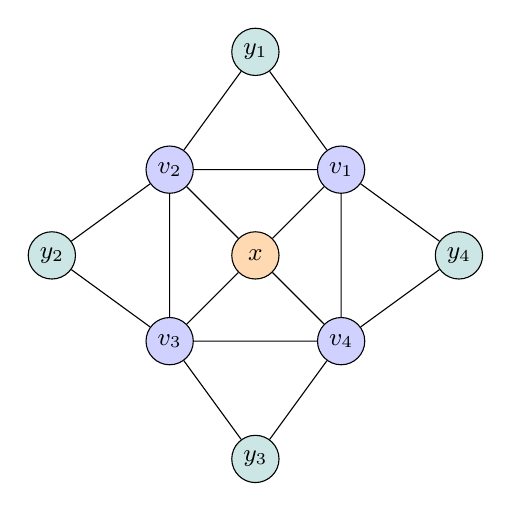
\begin{tikzpicture}[scale=1.1,vertex/.style={circle,draw,inner sep=2pt,minimum size=6mm,font=\small}]
\foreach \i/\ang in {1/45,2/135,3/225,4/315}{\node[vertex,fill=blue!18] (a\i) at (\ang:1.4) {\(v_\i\)};}
\foreach \i/\j in {1/2,2/3,3/4,4/1}{\draw (a\i)--(a\j);}
\node[vertex,fill=orange!30] (x) at (0,0){\(x\)};
\foreach \i in {1,2,3,4}{\draw (x)--(a\i);}
\foreach \i/\j/\ang in {1/2/90,2/3/180,3/4/270,4/1/0}{\node[vertex,fill=teal!20] (y\i) at (\ang:2.35){\(y_\i\)};\draw (y\i)--(a\i) (y\i)--(a\j);}
\end{tikzpicture}
\caption{The null example for \(d=2\). The same construction works for arbitrary \(d\).}\end{figure}

\section{Implicit coaffinity and Helly defect}\label{sec:defect}
\begin{theorem}[Region characterization]
For a finite family \(\mathcal R\subseteq\cl(X)\), a coaffine endomorphism of \(K(X)\) with images in \(\mathcal R\) exists exactly when there are regions \(U_A\subseteq V(X)\) for \(A\in\mathcal R\) satisfying
\[
 U_A\cap A=\varnothing,\quad U_A\cap U_B=\varnothing\ \text{if }A\cap B=\varnothing,
 \quad \forall Q\in\cl(X)\ \exists A:\ Q\subseteq U_A.
\]
\end{theorem}
\begin{proof}
Given a map, take each region to be the union of its fiber supports. Conversely choose any containing region for every source; the first condition ensures disjointness from its image, the second preserves intersections. The third ensures a choice everywhere.
\end{proof}
For a sampled finite collection of sources \(Q_i\), one can also avoid fixing an image pool: choose complete sets \(A_i\) disjoint from \(Q_i\), with every vertex of \(Q_i\) having a nonneighbor in \(A_i\), and with \(A_i\cap A_j\ne\varnothing\) whenever \(Q_i\cap Q_j\ne\varnothing\). This is equivalent to a coaffine morphism on the sampled induced subgraph: maximal extensions of the \(A_i\) remain disjoint from the corresponding sources and preserve their required intersections. An exhaustive negative result for a finite sample rules out a global coaffine map. A positive partial map need not extend. Region extension can greedily use \(U_B=(V(X)\setminus B)\setminus\bigcup_{A\cap B=\varnothing}U_A\). In practice the finite-pool and greedy-region methods covered training samples but not all independent test samples; no positive global map was found for the remaining cases.

For a coaffine \(f:K(X)\to K(X)\) and \(v\in V(X)\), define the pairwise intersecting family \(\mathcal F_v=\{T_{f(q)}:v\in T_q\}\). Its Helly defect occurs at \(v\) when \(\bigcap\mathcal F_v=\varnothing\). Write \(D(f)\) for the defect set and \(h_K(X)=\min_f |D(f)|\), with value infinity if no map exists.
\begin{theorem}[Defect localization]\label{thm:defect}
A coaffine \(f\) on \(K(X)\) induces a coaffine weak morphism \(g:X-D(f)\to X\) (coaffinity means \(g(v)\notin N_X[v]\)). Moreover, for every complete \(T\subseteq V(X)\), there exist \(a_x\notin N_X[x]\) for \(x\in T\cap D(f)\) such that \(g(T\setminus D(f))\cup\{a_x:x\in T\cap D(f)\}\) is complete.
\end{theorem}
\begin{proof}
For each nondefective vertex choose an element of the common intersection of its image-star. Adjacent source vertices occur in a common clique, so their choices are equal or adjacent. If a chosen image were in the closed neighborhood of its source, a clique containing both would have nondisjoint image, a contradiction. Extend \(T\) to a maximal complete \(q\). The maximal image clique \(f(q)\) contains all chosen images for nondefective vertices and is disjoint from \(q\). By maximality it has a nonneighbor of each omitted vertex \(x\in q\). Choose these witnesses simultaneously in the image clique.
\end{proof}
For clique-Helly \(X\), the defect is empty. Conversely a coaffine \(g:X\to X\) always induces a coaffine map of \(K(X)\) by extending the images of cliques: for every source vertex its image is a nonneighbor, so no extension can include it. Thus coaffine existence is equivalent on \(X\) and \(K(X)\) when \(X\) is clique-Helly.

\subsection{Graph 182}
The second pared host has 199 vertices, with \(\Delta(G_{182})\), \(\Delta(K(G_{182}))\) and the third topological level in the archived study contractible. It has no coaffine endomorphism: fixing vertex 41 at each of its only three possible images 101, 113, 176 gives contradictions by arc consistency. This excludes all retracts admitting coaffine endomorphisms at depth two. The first pared iterates of all twenty unresolved graphs were likewise certified non-coaffine in the archived search.

Fourteen induced source subsets admit no coaffine assignment into the 199-vertex host, the smallest found of size 18 and one inclusion-minimal example of size 25. By Theorem~\ref{thm:defect} the defect set must hit each of these subsets. Their common intersection is \(\{53,184\}\). Single-defect cases are ruled out by local extension constraints. Of \(\binom{199}{2}=19701\) possible pairs, 574 hit every obstruction; independent branching eliminates 559, and stronger tests eliminate fourteen more. The last pair \(\{53,184\}\) is excluded by the joint extension constraints from \(\{5,23,53,184\}\) and \(\{5,24,53,184\}\). All 574 exclusions and the fourteen original obstructions were replayed in the archived independent branching verifier (6,359 nodes in total). Consequently
\[
 h_K(P_2(G_{182}))\ge3.
\]
This includes the possibility of infinite defect. Neither the lower bound nor the absence of a coaffine endomorphism at depth two proves convergence. The combination of contractibility, enormous finite growth and stringent coaffine obstruction is a principal open phenomenon of the census.

\section{Implicit paring by replacement templates}\label{sec:paring}
The implicit clique graph in the current package stores all maximal-clique masks but avoids materializing edges. At the third level even storing all masks can be impossible. We instead reason about a symbolically represented family of surviving maximal completes.
\begin{definition}
For \(\mathcal F\subseteq\cl(X)\) and a nonempty complete \(T\), define
\[
 W_{\mathcal F}(T)=V(X)\setminus\bigcup_{Q\in\mathcal F,\ Q\cap T=\varnothing}Q,
 \qquad B(T)=V(X)\setminus\bigcap_{t\in T}N_X[t].
\]
Write \(W(T)\) for the full-family hull. The set \(B(T)\) consists of atoms incompatible with at least one template vertex.
\end{definition}
\begin{lemma}[Domination hull]
For \(A,Q\in\mathcal F\), \(Q\) is weakly dominated by \(A\) in the intersection graph of \(\mathcal F\) if and only if \(Q\subseteq W_{\mathcal F}(A)\).
\end{lemma}
\begin{proof}
Closed-neighborhood inclusion holds exactly when every survivor disjoint from \(A\) is disjoint from \(Q\), equivalent to the stated containment.
\end{proof}
To test hull membership for \(v\), ask for a maximal complete containing \(v\), disjoint from \(T\), and satisfying the current survivor constraints. A witness excludes \(v\) from the hull; exhaustive absence includes it. Relative hulls can grow after paring.
\begin{theorem}[Single replacement template]\label{thm:single}
For a nonempty complete \(T\), every clique in
\[
 \D_T=\{Q\in\cl(X):\ \varnothing\ne Q\cap B(T)\subseteq W(T)\}
\]
can be removed by ordinary folds while keeping every other clique.
\end{theorem}
\begin{proof}
Extend \((Q\setminus B(T))\cup T\) to a maximal complete \(A\). If a clique meets \(Q\) in its retained part it meets \(A\). If it meets a removed vertex, that vertex is in \(W(T)\), so the clique must intersect \(T\subseteq A\). Thus \(N[Q]\subseteq N[A]\). Since \(A\) contains \(T\), it avoids \(B(T)\), and therefore lies outside \(\D_T\). All such dominating cliques are retained, so one may delete the entire family in any order.
\end{proof}
\begin{figure}[ht]\centering
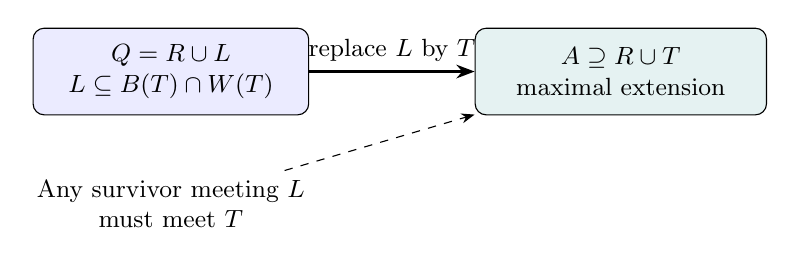
\begin{tikzpicture}[node distance=2.1cm,>=Stealth,every node/.style={font=\small}]
\node[draw,rounded corners,align=center,fill=blue!8,minimum width=3.5cm,minimum height=1.1cm] (q) {\(Q=R\cup L\)\\\(L\subseteq B(T)\cap W(T)\)};
\node[draw,rounded corners,align=center,fill=teal!10,right=of q,minimum width=3.7cm,minimum height=1.1cm] (a) {\(A\supseteq R\cup T\)\\maximal extension};
\draw[->,thick] (q)--node[above]{replace \(L\) by \(T\)} (a);
\node[below=7mm of q,align=center] (s) {Any survivor meeting \(L\)\\must meet \(T\)};
\draw[->,dashed] (s)--(a);
\end{tikzpicture}
\caption{One template certifies many ordinary folds with different dominators.}\end{figure}
\begin{corollary}[Compatible templates]
If \(\bigcup_iT_i\) is complete, then \(\bigcup_i\D_{T_i}\) can be removed simultaneously.
\end{corollary}
\begin{proof}
Each replacement inserts a new template and does not remove any vertex of previously inserted templates. Repeat until no eligible template remains. Transitivity of neighborhood inclusion gives a surviving dominator for each original deleted vertex.
\end{proof}
The condition can be relaxed using a common ranking of atoms.
\begin{theorem}[Lexicographic replacement]\label{thm:rank}
Let \(\succ\) be a total order on \(V(X)\). For each template \(T_i\) assume every vertex \(v\in B(T_i)\cap W(T_i)\) has a nonadjacent witness \(t\in T_i\) with \(t\succ v\). Then the union of the deletion families admits a simultaneous ordinary folding retraction onto its complement, nondecreasing in the lexicographic order of subsets (highest-ranked differing atom wins).
\end{theorem}
\begin{proof}
Each replacement removes only eligible incompatible vertices. Every removed vertex has a higher-ranked inserted witness, which was not in the source clique. Hence the largest atom of the symmetric difference is inserted, not removed. Extension to a clique only adds atoms. Each replacement strictly increases lexicographic rank while producing a dominating vertex. Finiteness ensures termination outside the union. The terminal vertex dominates the original by transitivity, so all deleted vertices can be folded onto surviving ones. The map fixes survivors and is rank nondecreasing.
\end{proof}
The ranking condition is decidable by greedy highest-first placement. Place an unranked atom when for every requirement attached to it at least one witness has already been placed. Eligibility is monotone, so placing any eligible atom cannot destroy a feasible order; if none is eligible, no feasible order exists. This is a necessary-and-sufficient test of the \emph{ranking condition}, not of simultaneous parability.
\begin{theorem}[Successive implicit paring]\label{thm:relative}
Suppose previous rounds yield a lexicographically nondecreasing retraction \(r\) of the full clique graph onto the intersection graph of the surviving family \(\mathcal F\). Use relative hulls \(W_{\mathcal F}(T_i)\) and the same ranking satisfying Theorem~\ref{thm:rank}'s witness condition. Then the eligible members of \(\mathcal F\) can be deleted by ordinary folds, and the composite retraction is still nondecreasing.
\end{theorem}
\begin{proof}
For eligible \(Q\in\mathcal F\), replace its incompatible atoms and extend to a full clique \(A\), possibly outside \(\mathcal F\). Every survivor meeting \(Q\) meets \(A\), by the relative hull property; since \(r\) fixes survivors, every such survivor is equal or adjacent to \(r(A)\). The latter dominates \(Q\) within \(\mathcal F\). The replacement strictly increases rank and \(r\) does not decrease it. Iterate to a survivor outside the new union. This yields the claimed ordinary folds and monotone composite.
\end{proof}
If \(L_i=B(T_i)\cap W_{\mathcal F}(T_i)\) and \(F_i=B(T_i)\setminus W_{\mathcal F}(T_i)\), survivors of a new round are characterized by the additional clauses \(\neg z_v\lor\bigvee_{w\in F_i}z_w\) for \(v\in L_i\). The empty disjunction is false. This permits another round without enumerating survivors. It does not guarantee that the template family discovers every possible domination.

\subsection{Application and experimental evidence}
In graph 182, the first hull searches identified 237 distinct dominated vertices (one clique dominated 69); graph 441 yielded three. The original 14 compatible templates gave a certified lower bound of 40,275,869 removable cliques. A direct template discovery method starts with a complete hitting every clique containing an incompatible vertex, and removes template atoms while preserving the hitting property. Subsequent searches gave a compatible family of 40 and finally a lexicographically ranked family of 77 (822 incompatible template pairs). All 77 hulls and the common order were replayed in the archive with 9,825 branching nodes. The corresponding four templates of graph 441 have five incompatible pairs yet admit a common ranking.

\begin{center}\begin{tabular}{lr}\toprule
Family or disjoint increment&certified removable vertices\\\midrule
14 compatible templates&40,275,869\\
40 compatible templates&99,340,876\\
Extra 37 templates, excluding the previous 40&3,175,406\\\midrule
77 ranked templates, combined lower bound&102,516,282\\\bottomrule\end{tabular}\end{center}
The last two summands were obtained by separate bounded bitset enumerations of disjoint sets (650 million and 250 million search nodes). The full counting problem exceeded resources; these are not exact totals, and the remaining graph is not known to be stiff. The archived exhaustive atlas validation covered 1,251 graphs of orders two to seven, 2,260 relative templates, 1,871 folds, 936 rounds, 91 multi-round graphs and 155 genuinely enlarged useful relative hulls, with no disagreements. On graph 182 itself the new discovered hulls so far already held before paring. The numerical size of a deletion family alone is not a convergence or divergence certificate.

\section{What remains open and how to continue}
The census is unchanged since the graph 308 result. Three particularly important lessons are: an enormous induced octahedron is not enough; complement domination is necessary but not sufficient; and a successful paring strategy must characterize the survivor family, not merely count many removable vertices. Exact negative tests for particular octahedra, finite pools, coaffine maps, local regions and low Helly-defect sets are not convergence tests.

For the remaining twenty graphs the priorities are (i) implicit paring to a sufficiently tractable survivor family, with new relative hulls and proofs of completeness where possible; (ii) nonoctahedral expansive coaffine structures, without imposing an octahedral stable image; (iii) covering-based or other admissible-map divergence criteria \cite{relations}; (iv) searching the less investigated hosts rather than repeatedly repairing the three exhausted symbolic target families; and (v) treating graph 182 as a distinct topological and dynamical question. The lexicographic replacement method and region-based SAT encodings are promising reusable extensions of \code{pycliques}. They are not yet part of the current production APIs. The current package's \code{ImplicitCliqueGraph} stores the full family of maximal cliques as masks; it does not implement the exponentially implicit survivor family described here.

\appendix
\section{Research provenance and computational proof obligations}
The companion Org document provides all recorded behavior groups, executable package calls, explicit certificate checks and a fallback archive index. Key archives available in the continuation include (filenames are literal):
\begin{longtable}{p{.48\linewidth}p{.44\linewidth}}
\toprule Archive or ledger & Main content\\\midrule\endhead
\path{updated_behavior_ledger.csv} & Full classification stage and source.\\
\path{cubic14_complete_homotopy_transitions.csv} & 540 exact recorded wedge transitions.\\
\path{cubic_expansive_census_research.zip} & Earlier stable-image certificates and point reductions; four historical records not replayed.\\
\path{cubic14_final_twelve_certificates.zip} & Earlier final homotopy proofs.\\
\path{cubic_sat_research.zip}, \path{cubic_incidence_post67_research.zip} & Stage-two SAT and cut-search work; earlier project archives.\\
\path{certificate308.json} & 22 cuts, support data and projection; independently checked in preparation of this survey.\\
\path{cubic14_local_repair_research.zip} & Recovered near-retractions, local repair and core bounds.\\
\path{cubic14_enlarged_targets_research.zip} & Enlarged targets and anchored coaffine tests.\\
\path{cubic14_implicit_third_iterate_research.zip} & Implicit SAT, induced growth witnesses and non-coaffinity of 182.\\
\path{cubic14_implicit_domination_research.zip} & Hulls and switching; obstruction cliques.\\
\path{cubic14_finite_pool_research.zip} & Variable-cut pool formulation and exact pool obstructions.\\
\path{cubic14_defect_three_research.zip} & Local obstruction hypergraph and complete defect-three verifier.\\
\path{cubic14_symbolic_lift_research.zip} & Symbolic orientation counts and forced-transversal certificates.\\
\path{cubic14_mandatory_shores_research.zip} & Exact impossibility of the three lifted families.\\
\path{cubic14_ranked_paring_research.zip} & 77-template proof, ranking, count inputs and independent verifiers.\\\bottomrule
\end{longtable}
The first archived ZIPs are referenced for provenance; raw access to some earlier project files was unavailable during survey preparation. The later archives listed above were available in the conversation and their README/verifier sources were inspected. We do not promote timeouts to negative results. In every positive case the relevant proof obligations are: reconstruct the original graph and all required clique families; verify folds; check every edge of a claimed morphism and fixation of target vertices; check coaffinity and invariance for expansive witnesses; or verify an actual homotopy certificate. The current package source inspected includes commit \code{e1e9ed04f5c1f962a5f7e70312fb8df16e5a6a78} in search results, with the subsequently fetched default-branch APIs described in the Org companion. Native search budgets and solver versions can affect discovery, but never the verification of a saved map. We distinguish the archived ledger from fresh experiments; no new behavior verdict is claimed here.

\begin{thebibliography}{99}
\bibitem{regular} R. Villarroel-Flores, On the clique behavior and Hellyness of the complements of regular graphs, \emph{Discrete Mathematics} 346 (2023), 113230. \href{https://doi.org/10.1016/j.disc.2022.113230}{doi:10.1016/j.disc.2022.113230}.
\bibitem{lagos} R. Villarroel-Flores, The clique behavior of the complement of cubic graphs, LAGOS 2023 conference manuscript (archived eight-page draft; not cited here as a verified final publication).
\bibitem{expansive} F. Larrión, V. Neumann-Lara, M. A. Pizaña, On expansive graphs, \emph{European Journal of Combinatorics} 30 (2009), 372--379. \href{https://doi.org/10.1016/j.ejc.2008.05.005}{doi:10.1016/j.ejc.2008.05.005}.
\bibitem{relations} F. Larrión, V. Neumann-Lara, M. A. Pizaña, Graph relations, clique divergence and surface triangulations, \emph{Journal of Graph Theory} 51 (2006), 110--122. \href{https://doi.org/10.1002/jgt.20126}{doi:10.1002/jgt.20126}.
\bibitem{dismantling} M. E. Frías-Armenta, V. Neumann-Lara, M. A. Pizaña, Dismantlings and iterated clique graphs, \emph{Discrete Mathematics} 282 (2004), 263--265.
\bibitem{contraction} M. E. Frías-Armenta, F. Larrión, V. Neumann-Lara, M. A. Pizaña, Edge contraction and edge removal on iterated clique graphs, \emph{Discrete Applied Mathematics} (2013). \href{https://doi.org/10.1016/j.dam.2013.02.003}{doi:10.1016/j.dam.2013.02.003}.
\bibitem{collapses} F. Larrión, M. A. Pizaña, R. Villarroel-Flores, Equivariant collapses and the homotopy type of iterated clique graphs, \emph{Discrete Mathematics} (2008). \href{https://doi.org/10.1016/j.disc.2007.06.021}{doi:10.1016/j.disc.2007.06.021}.
\bibitem{escalante} F. Escalante, Über iterierte Clique-Graphen, \emph{Abhandlungen aus dem Mathematischen Seminar der Universität Hamburg} 39 (1973), 59--68.
\bibitem{hog} K. Coolsaet, S. D'hondt, J. Goedgebeur, House of Graphs 2.0: A database of interesting graphs and more, \emph{Discrete Applied Mathematics} 325 (2023), 97--107. \url{https://houseofgraphs.org/Cubic}.
\bibitem{forman} R. Forman, Morse theory for cell complexes, \emph{Advances in Mathematics} 134 (1998), 90--145.
\bibitem{dong} X. Dong, Topology of bounded-degree graph complexes, \emph{Journal of Algebra} (2003). \href{https://doi.org/10.1016/S0021-8693(03)00024-3}{doi:10.1016/S0021-8693(03)00024-3}.
\bibitem{hatcher} A. Hatcher, \emph{Algebraic Topology}, Cambridge University Press, 2002. \url{https://pi.math.cornell.edu/~hatcher/AT/ATpage.html}.
\bibitem{software} \emph{pycliques-project}, Python workspace: pycliques, pycombtop, pyg6data. \url{https://github.com/rvf0068/pycliques-project}. See the package documentation and the research scripts referenced in the companion workbook.
\end{thebibliography}
\end{document}
